\documentclass[a4paper,10pt]{article}
\usepackage[margin=0.8in,top=0.5in]{geometry}  % Reduced top margin from 0.8in to 0.5in
\usepackage{enumitem}
\usepackage{hyperref}
\usepackage{xeCJK} % For CJK fonts
\usepackage{tabularx}
\usepackage{graphicx} % For including images
\usepackage{pdfpages} % Add pdf file
\usepackage{xcolor} % For color

\hypersetup{
    colorlinks=true,
    linkcolor=blue,
    urlcolor=blue
}

% macros
\newcommand{\coloredsection}[1]{\section*{\textcolor{blue!70!black}{#1}}}


\begin{document}
\sloppy % Allow line breaks in long words

% Title and photo layout
\begin{tabularx}{\textwidth}{lXr}
    \begin{minipage}[c]{0.6\textwidth} % Change [t] to [c] for vertical alignment
        \vspace{0.5cm}
        {\LARGE \textbf{Tsung-Yi Ma}} \\
        \vspace{0.2cm}
        
        \noindent
        
\includegraphics[height=1em]{icon/gmail.jpg}
        \href{mailto:johnny880319@gmail.com}{johnny880319@gmail.com} \\  % Changed symbol
        
\includegraphics[height=1em]{icon/linkedin.png}
        \href{https://www.linkedin.com/in/tsung-yi-ma-44bb6a268}{Tsung-Yi Ma} \\  % Added LinkedIn symbol
        
\includegraphics[height=1em]{icon/moblie_phone.jpg}
        0979712027 \\  % Added phone symbol
    \end{minipage} &
    &
    \begin{minipage}[c]{0.3\textwidth} % Change [t] to [c] for vertical alignment
        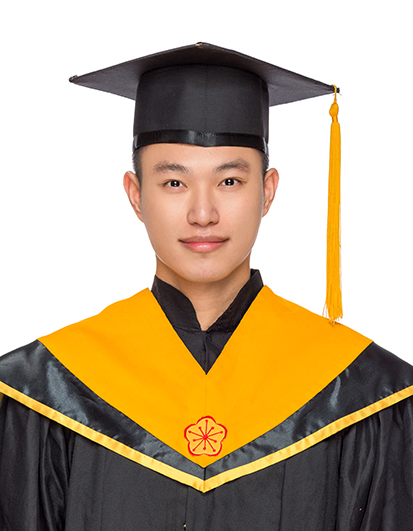
\includegraphics[width=0.6\textwidth]{picture/master_graduation_photo.jpeg} % Adjusted image size
    \end{minipage}
\end{tabularx}


\vspace{0.5cm}
\noindent
\coloredsection{Profile}
R\&D Engineer with a strong background in mathematics and hands-on experience in optimization, mathematical modeling, and applied AI. Passionate about using math and algorithms to solve real-world problems, especially in automation and intelligent systems.


\vspace{0.5cm}
\coloredsection{Work Experience}
\begin{tabularx}{\textwidth}{Xr}
    \textbf{Research \& Development Engineer, ASUSTEK COMPUTER INC.} & \textit{2023--present} \\
\end{tabularx}
\begin{itemize}[leftmargin=30pt]
    \item \textbf{Production Scheduling Optimization System:}
    \begin{itemize}
        \item Designed and optimized mathematical models (e.g., MIP/LP) using Python and CPLEX/SCIP for production scheduling problems.
        \item Reduced execution time from over 24 hours to under 1 hour by minimizing model size and restructuring constraints.
        \item Simulations showed that under raw material shortages, the system increased output by 10\% compared to the traditional FIFO method.
    \end{itemize}
    \item \textbf{GAI Recruiter System:}
    \begin{itemize}
        \item Implemented streaming speech recognition using a sliding window approach, reducing recognition latency from audio-length-dependent to a constant delay.
        \item Adjusted inference parameters such as \texttt{vad\_filter}, \texttt{beam\_size}, and \texttt{no\_repeat\_ngram\_size} based on experiments and online resources to reduce hallucination and improve transcription quality.
    \end{itemize}
\end{itemize}

\coloredsection{Education}
\begin{tabularx}{\textwidth}{Xr}
    \textbf{Master of Mathematics, NATIONAL TAIWAN UNIVERSITY} & \textit{2021--2023} \\
\end{tabularx}
\begin{itemize}[leftmargin=30pt]
    \item \textbf{Master's Thesis:} Introduction to the Ising Model and the Ising Model with Disorders:
    \begin{itemize}
        \item Applied rigorous mathematical analysis to study statistical physics models, including phase transitions and disorder effects.
    \end{itemize}
    \item \textbf{Teaching Assistant:} Mathematical Analysis, Probability Theory.
    \item \textbf{Courses:}
    \begin{itemize}
        \item Data Structure and Algorithm, Machine Learning: Completed programming tasks using Python and C.
        \item Mathematics: Completed over 100 credits of math courses during undergraduate and master's studies.
    \end{itemize}
\end{itemize}

\noindent
\begin{tabularx}{\textwidth}{Xr}
    \textbf{Bachelor of Mathematics, NATIONAL TAIWAN UNIVERSITY} & \textit{2017--2021} \\
\end{tabularx}
\begin{itemize}[leftmargin=30pt]
    \item \textbf{NCTS Undergraduate Research Program:} Noncommutative Probability Theory:
    \begin{itemize}
        \item Participated in a study group hosted by the Quantum Computing Research Center of Hon Hai Research Institute (鴻海研究院).
    \end{itemize}
\end{itemize}

\noindent
\begin{tabularx}{\textwidth}{Xr}
    \textbf{Class of Science (科學班), TAIPEI MUNICIPAL CHIEN KUO HIGH SCHOOL} & \textit{2014--2017} \\
\end{tabularx}

\coloredsection{Awards}
\begin{itemize}[leftmargin=30pt]
    \item The Phi Tau Phi (斐陶斐) Scholastic Honor Society of the Republic of China Honorary Membership.
    \item Symposium for Young Analysts at National Central University.
    \item NCTS Undergraduate Summer Research Program.
\end{itemize}

\coloredsection{Skills}
\begin{itemize}[leftmargin=30pt]
    \item Programming: Python (daily use), C++ (LeetCode practice), C (academic)
    \item Tools: Git, Linux, SQL, \LaTeX
    \item Web: Basic HTML, CSS, JavaScript (used in AI demo interfaces)
    \item Other: Diabolo, juggling, unicycling — keeps me balanced inside and outside work
\end{itemize}


\coloredsection{Appendix}

    \begin{center}
        \begin{tabular}{cc}
            \fbox{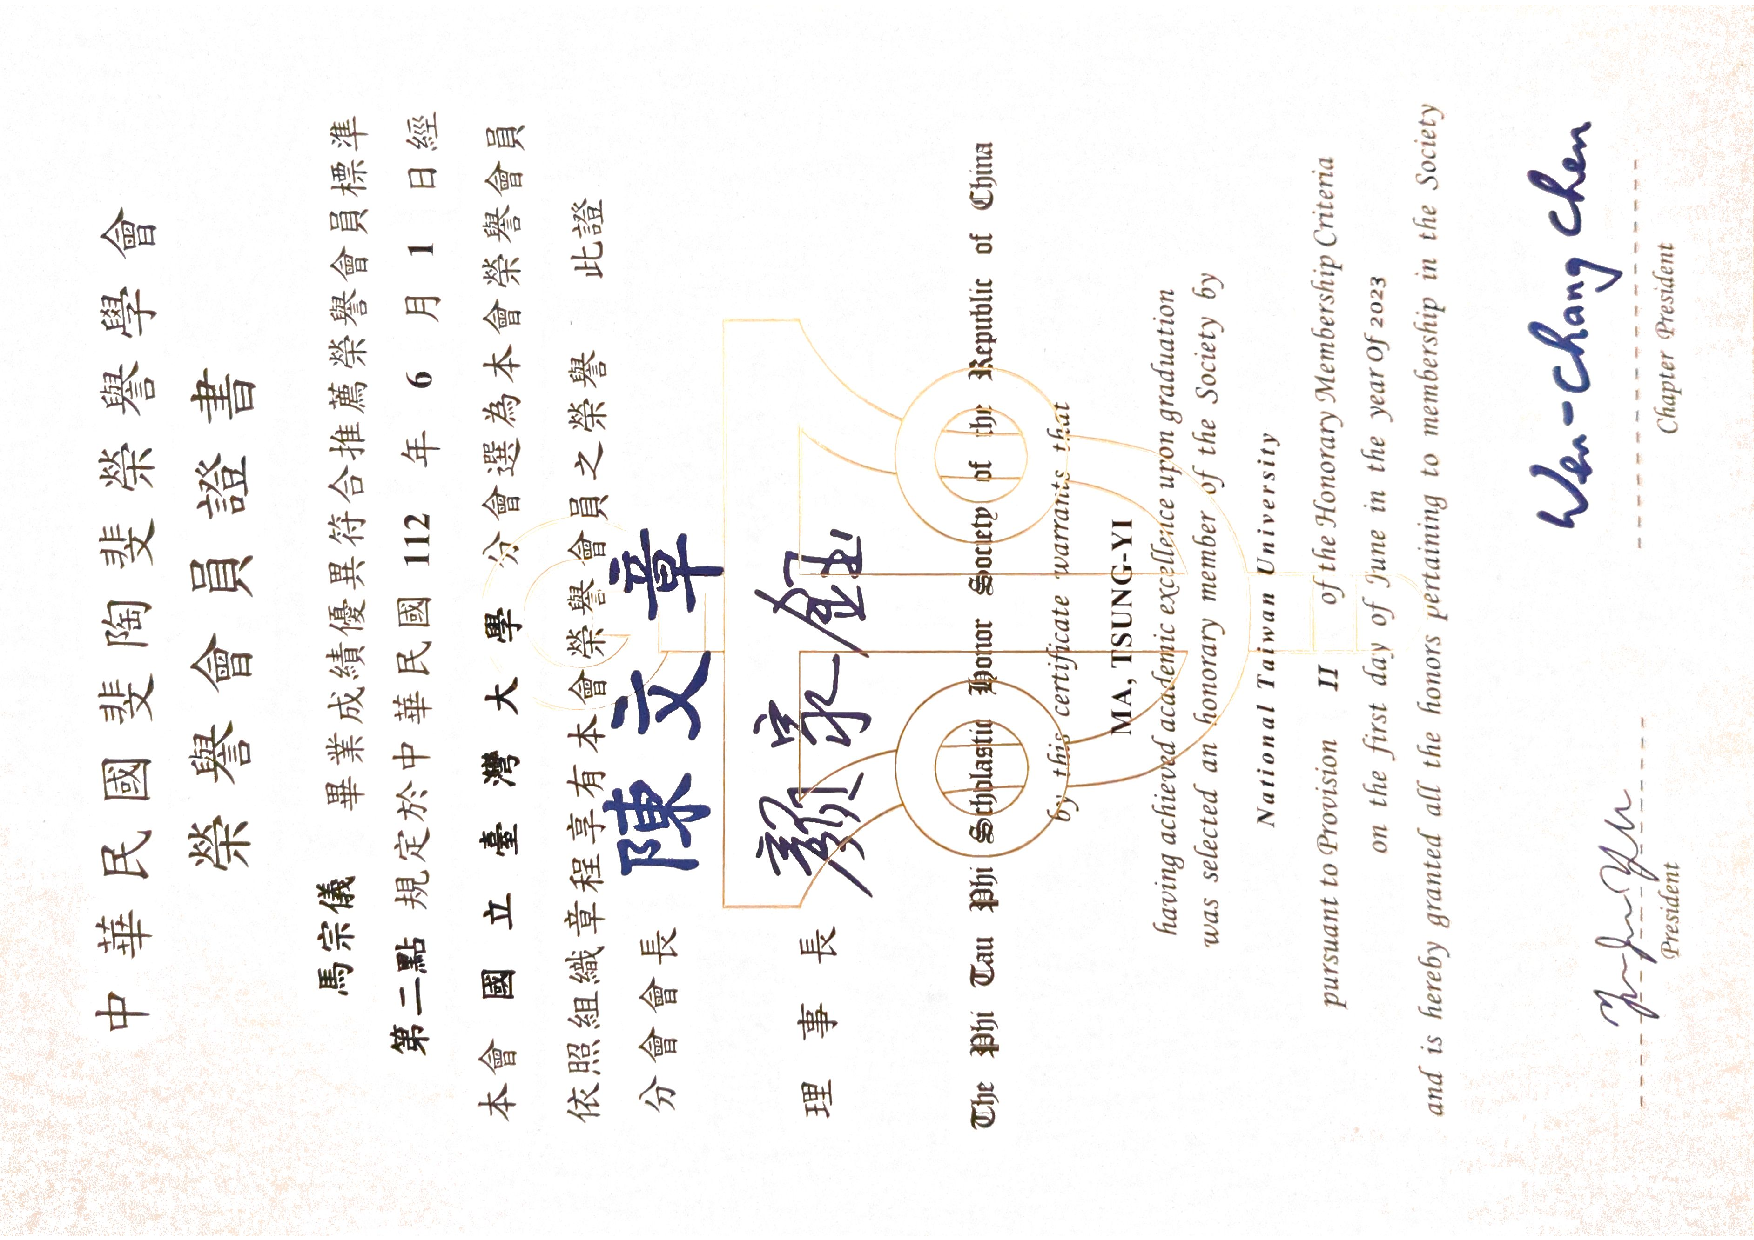
\includegraphics[page=1,width=0.45\textwidth]{pdf_data/Phi_Tau_Phi.pdf}} &
            \fbox{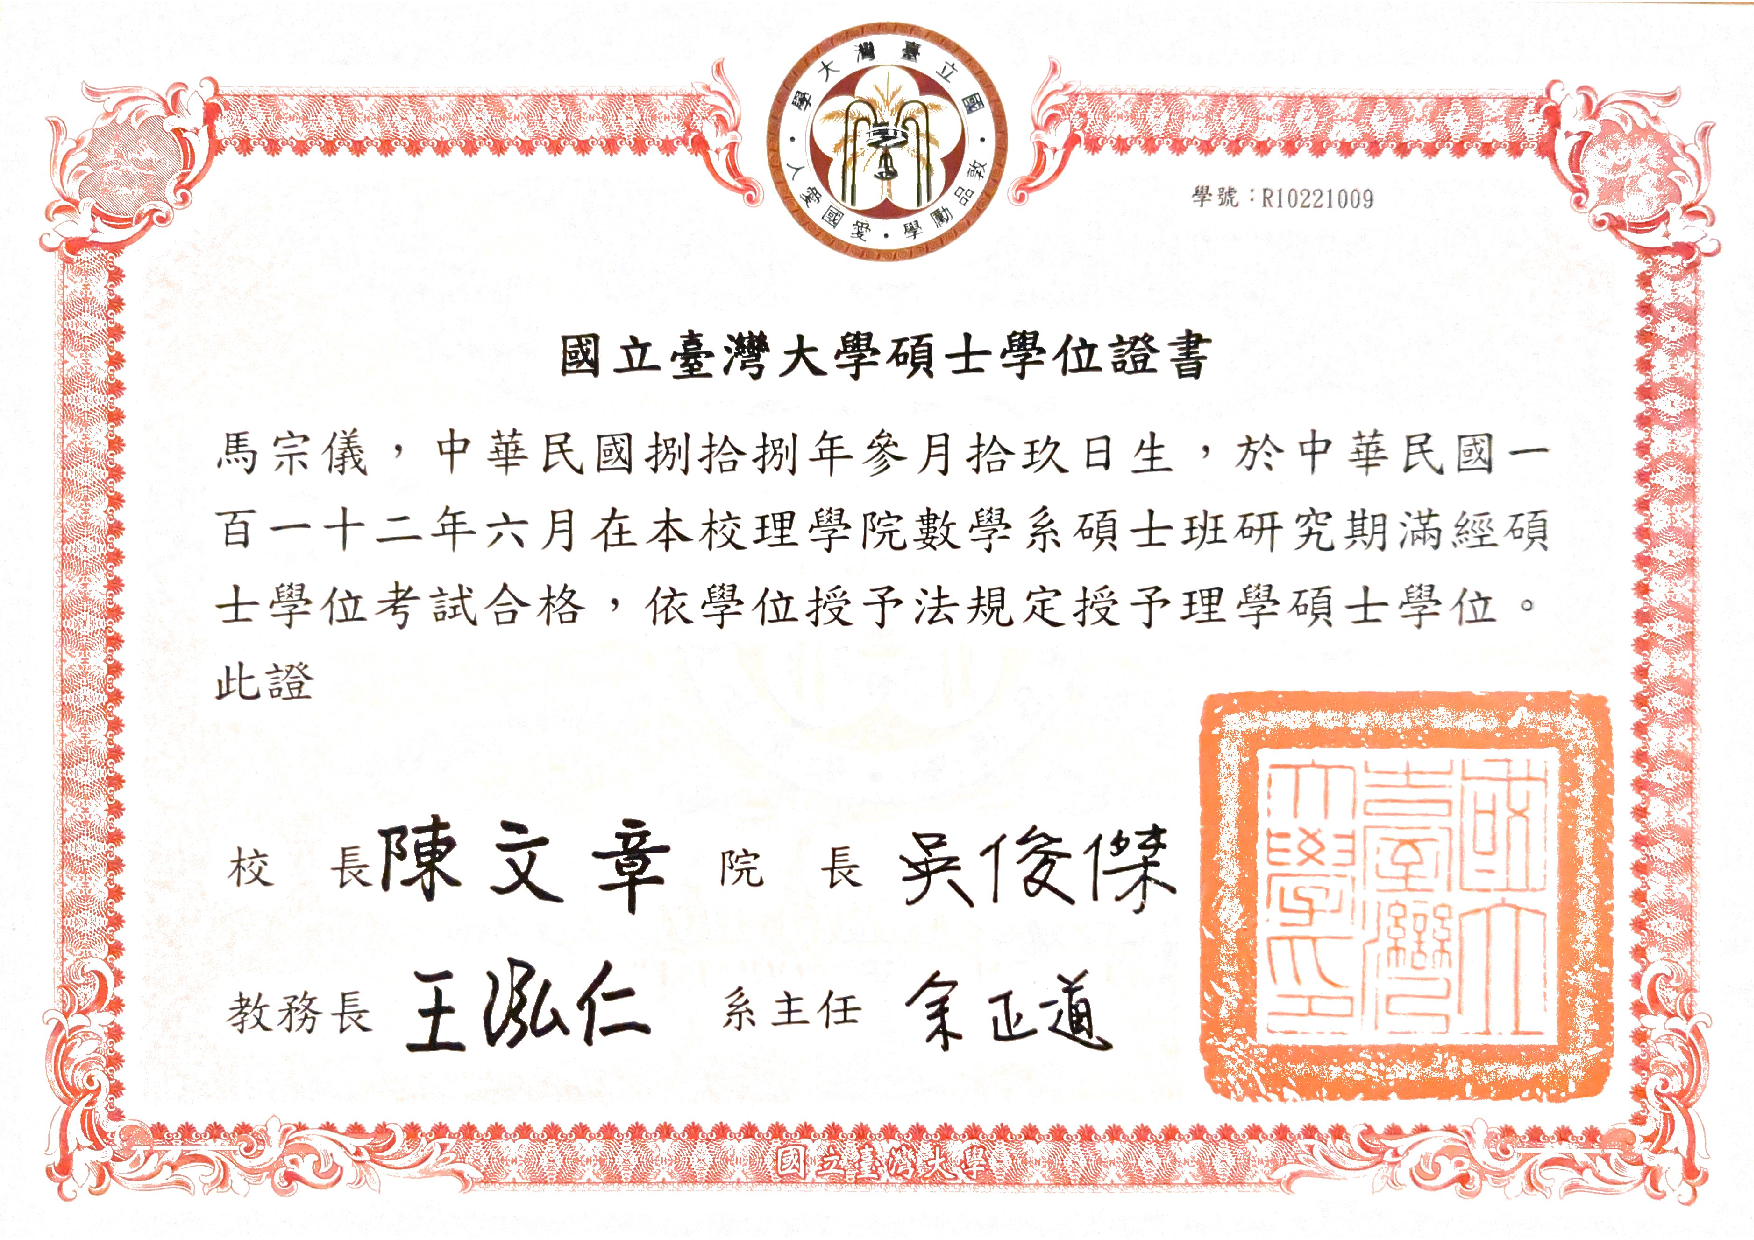
\includegraphics[page=1,width=0.45\textwidth]{pdf_data/master_certificate.pdf}} \\[1ex]
            \fbox{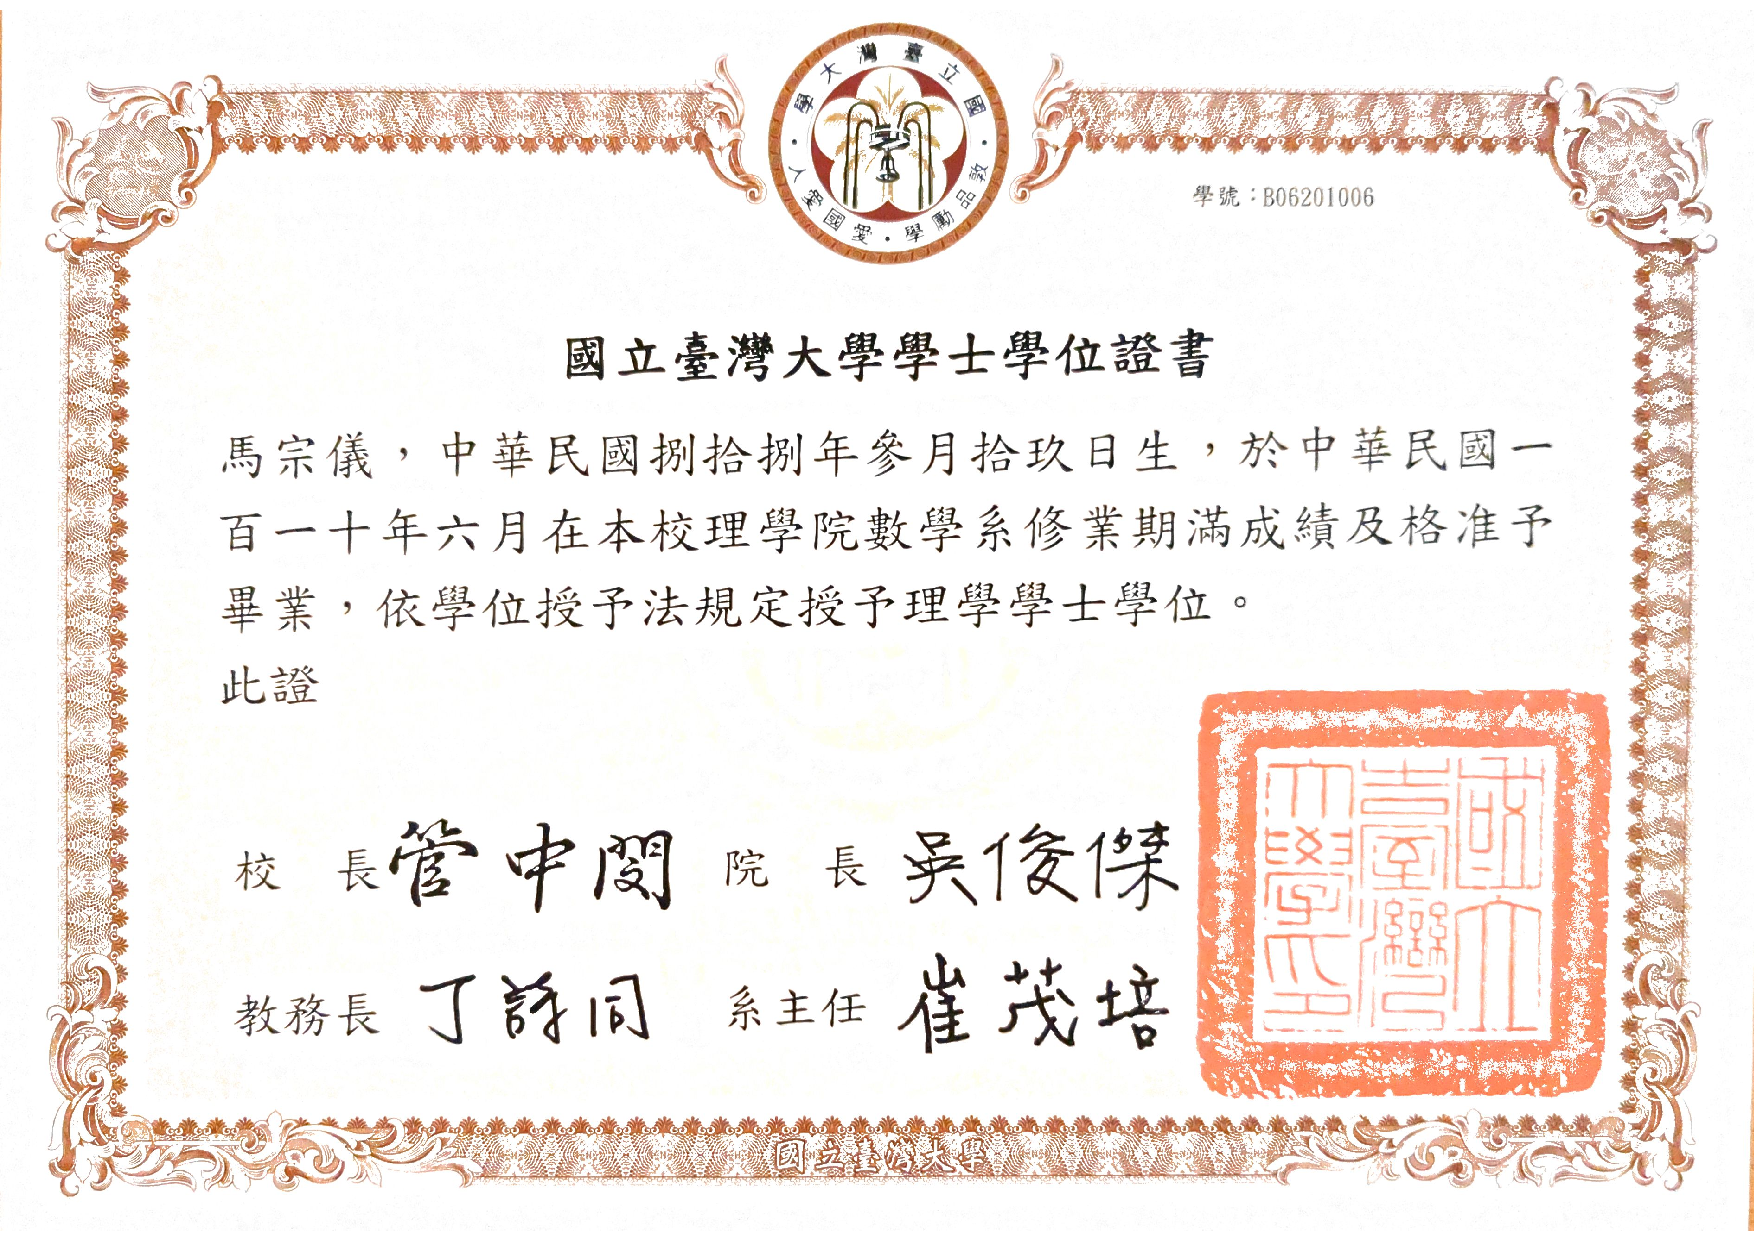
\includegraphics[page=1,width=0.45\textwidth]{pdf_data/bachelor_certificate.pdf}} &
            \fbox{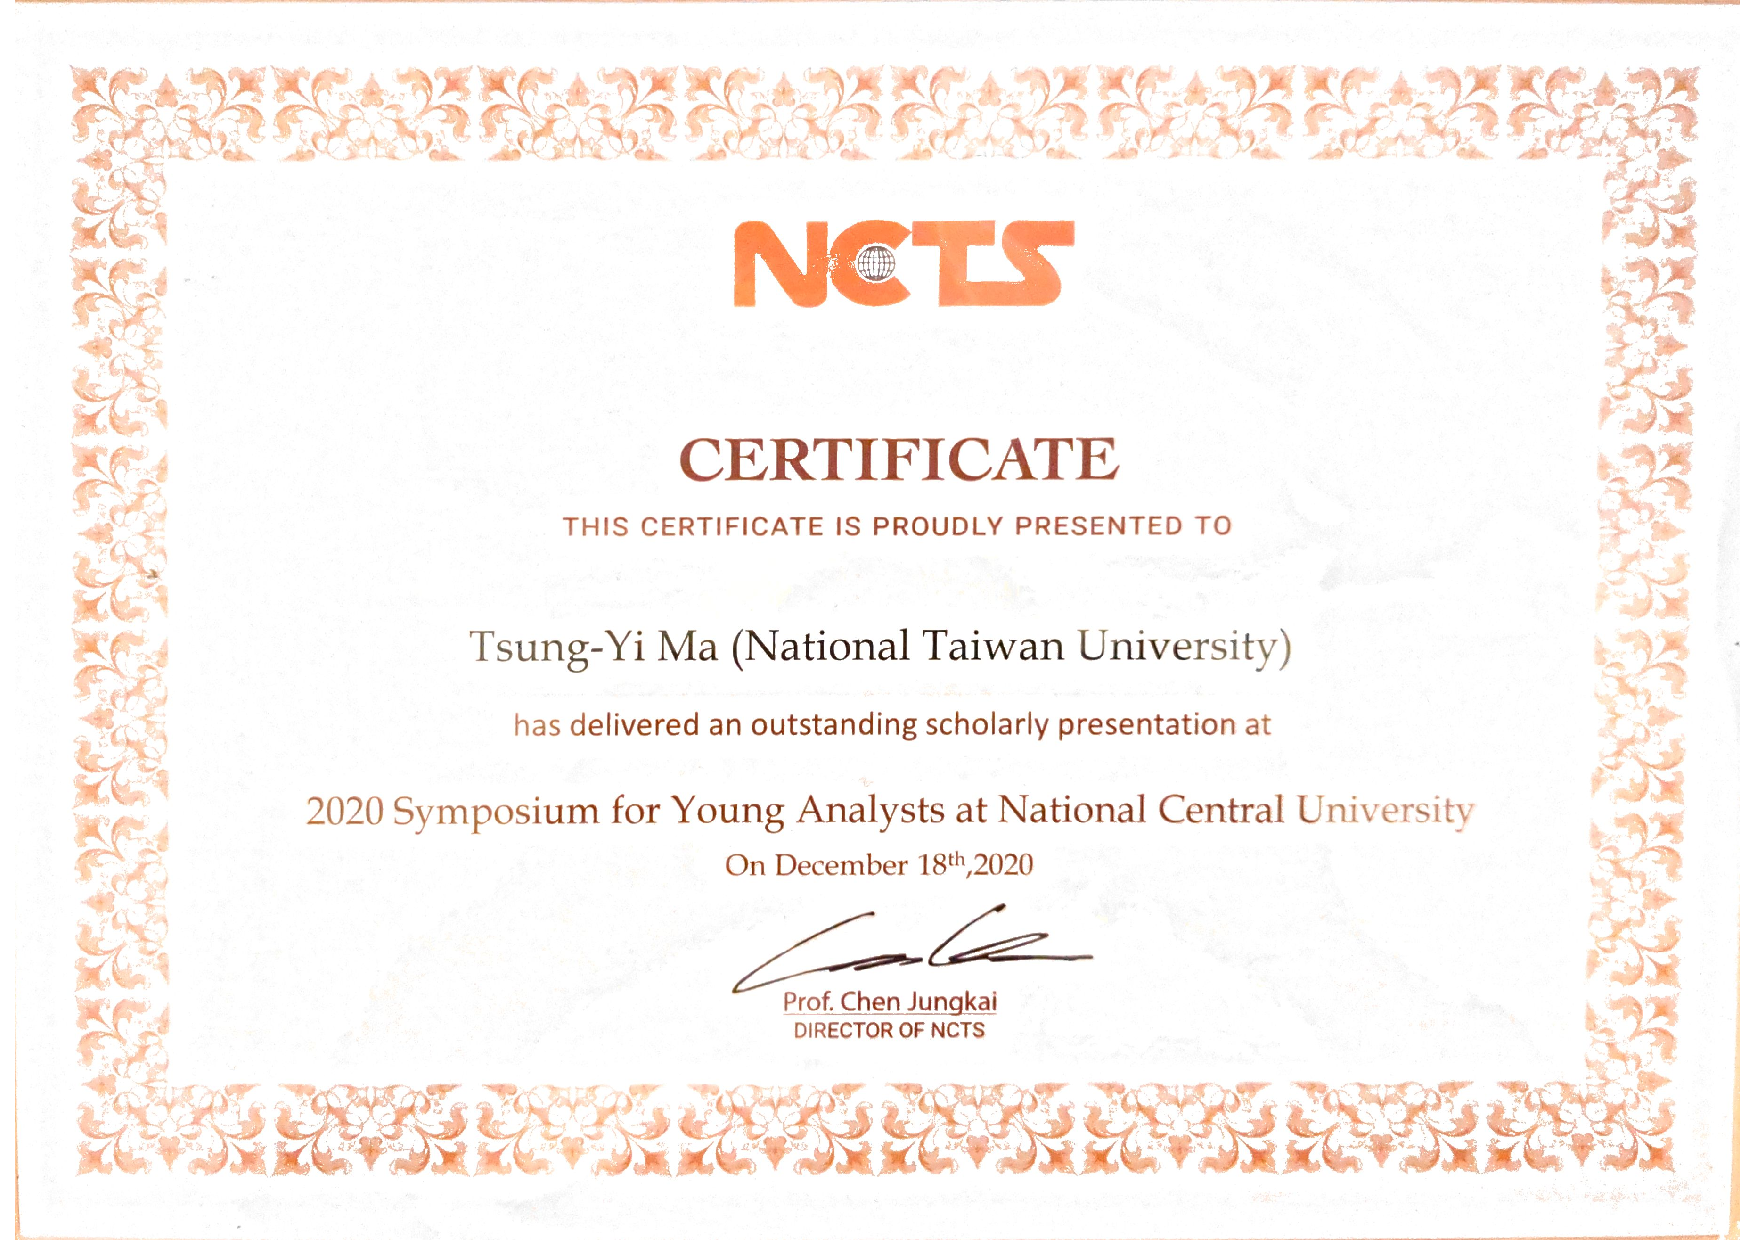
\includegraphics[page=1,width=0.45\textwidth]{pdf_data/symposium_young_analysts.pdf}} \\[1ex]
            \fbox{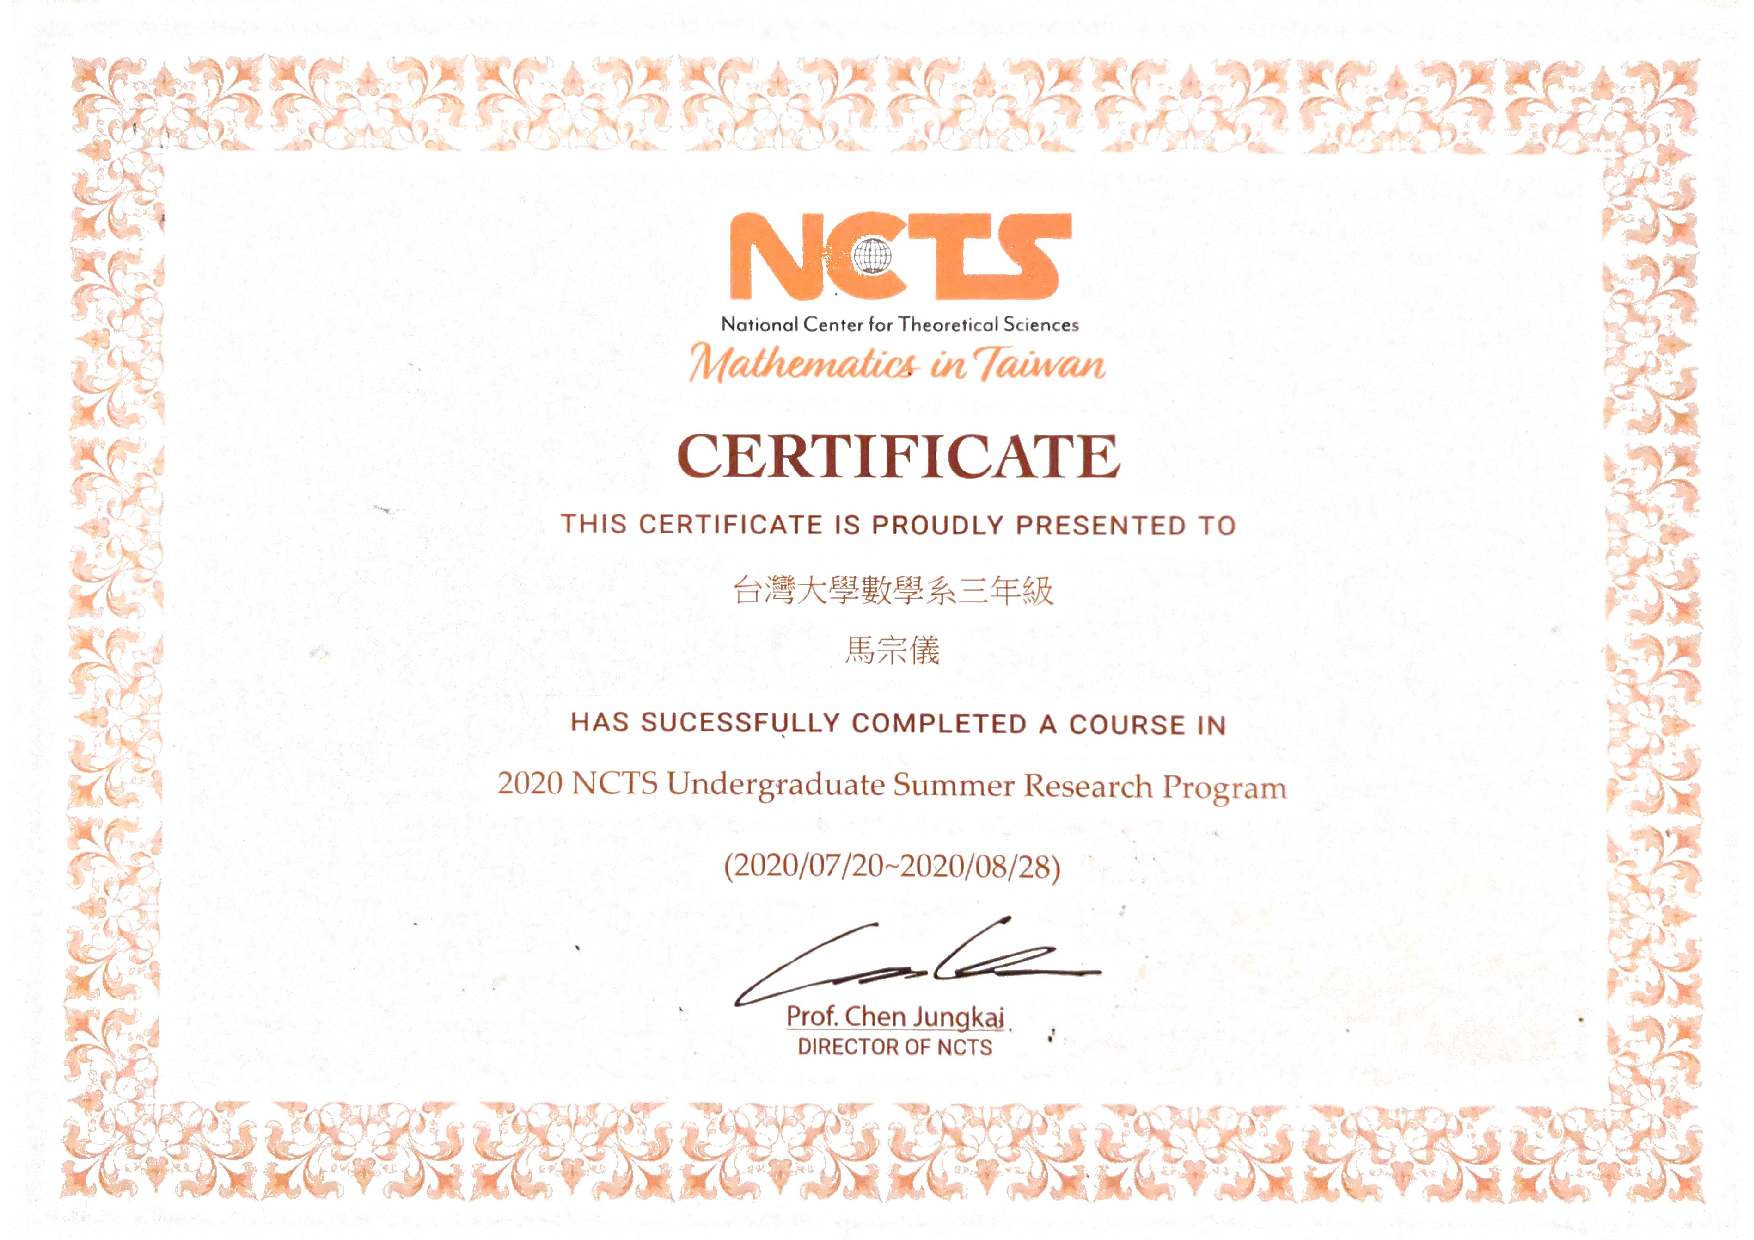
\includegraphics[page=1,width=0.45\textwidth]{pdf_data/NCTS_USRP.pdf}} &
            \fbox{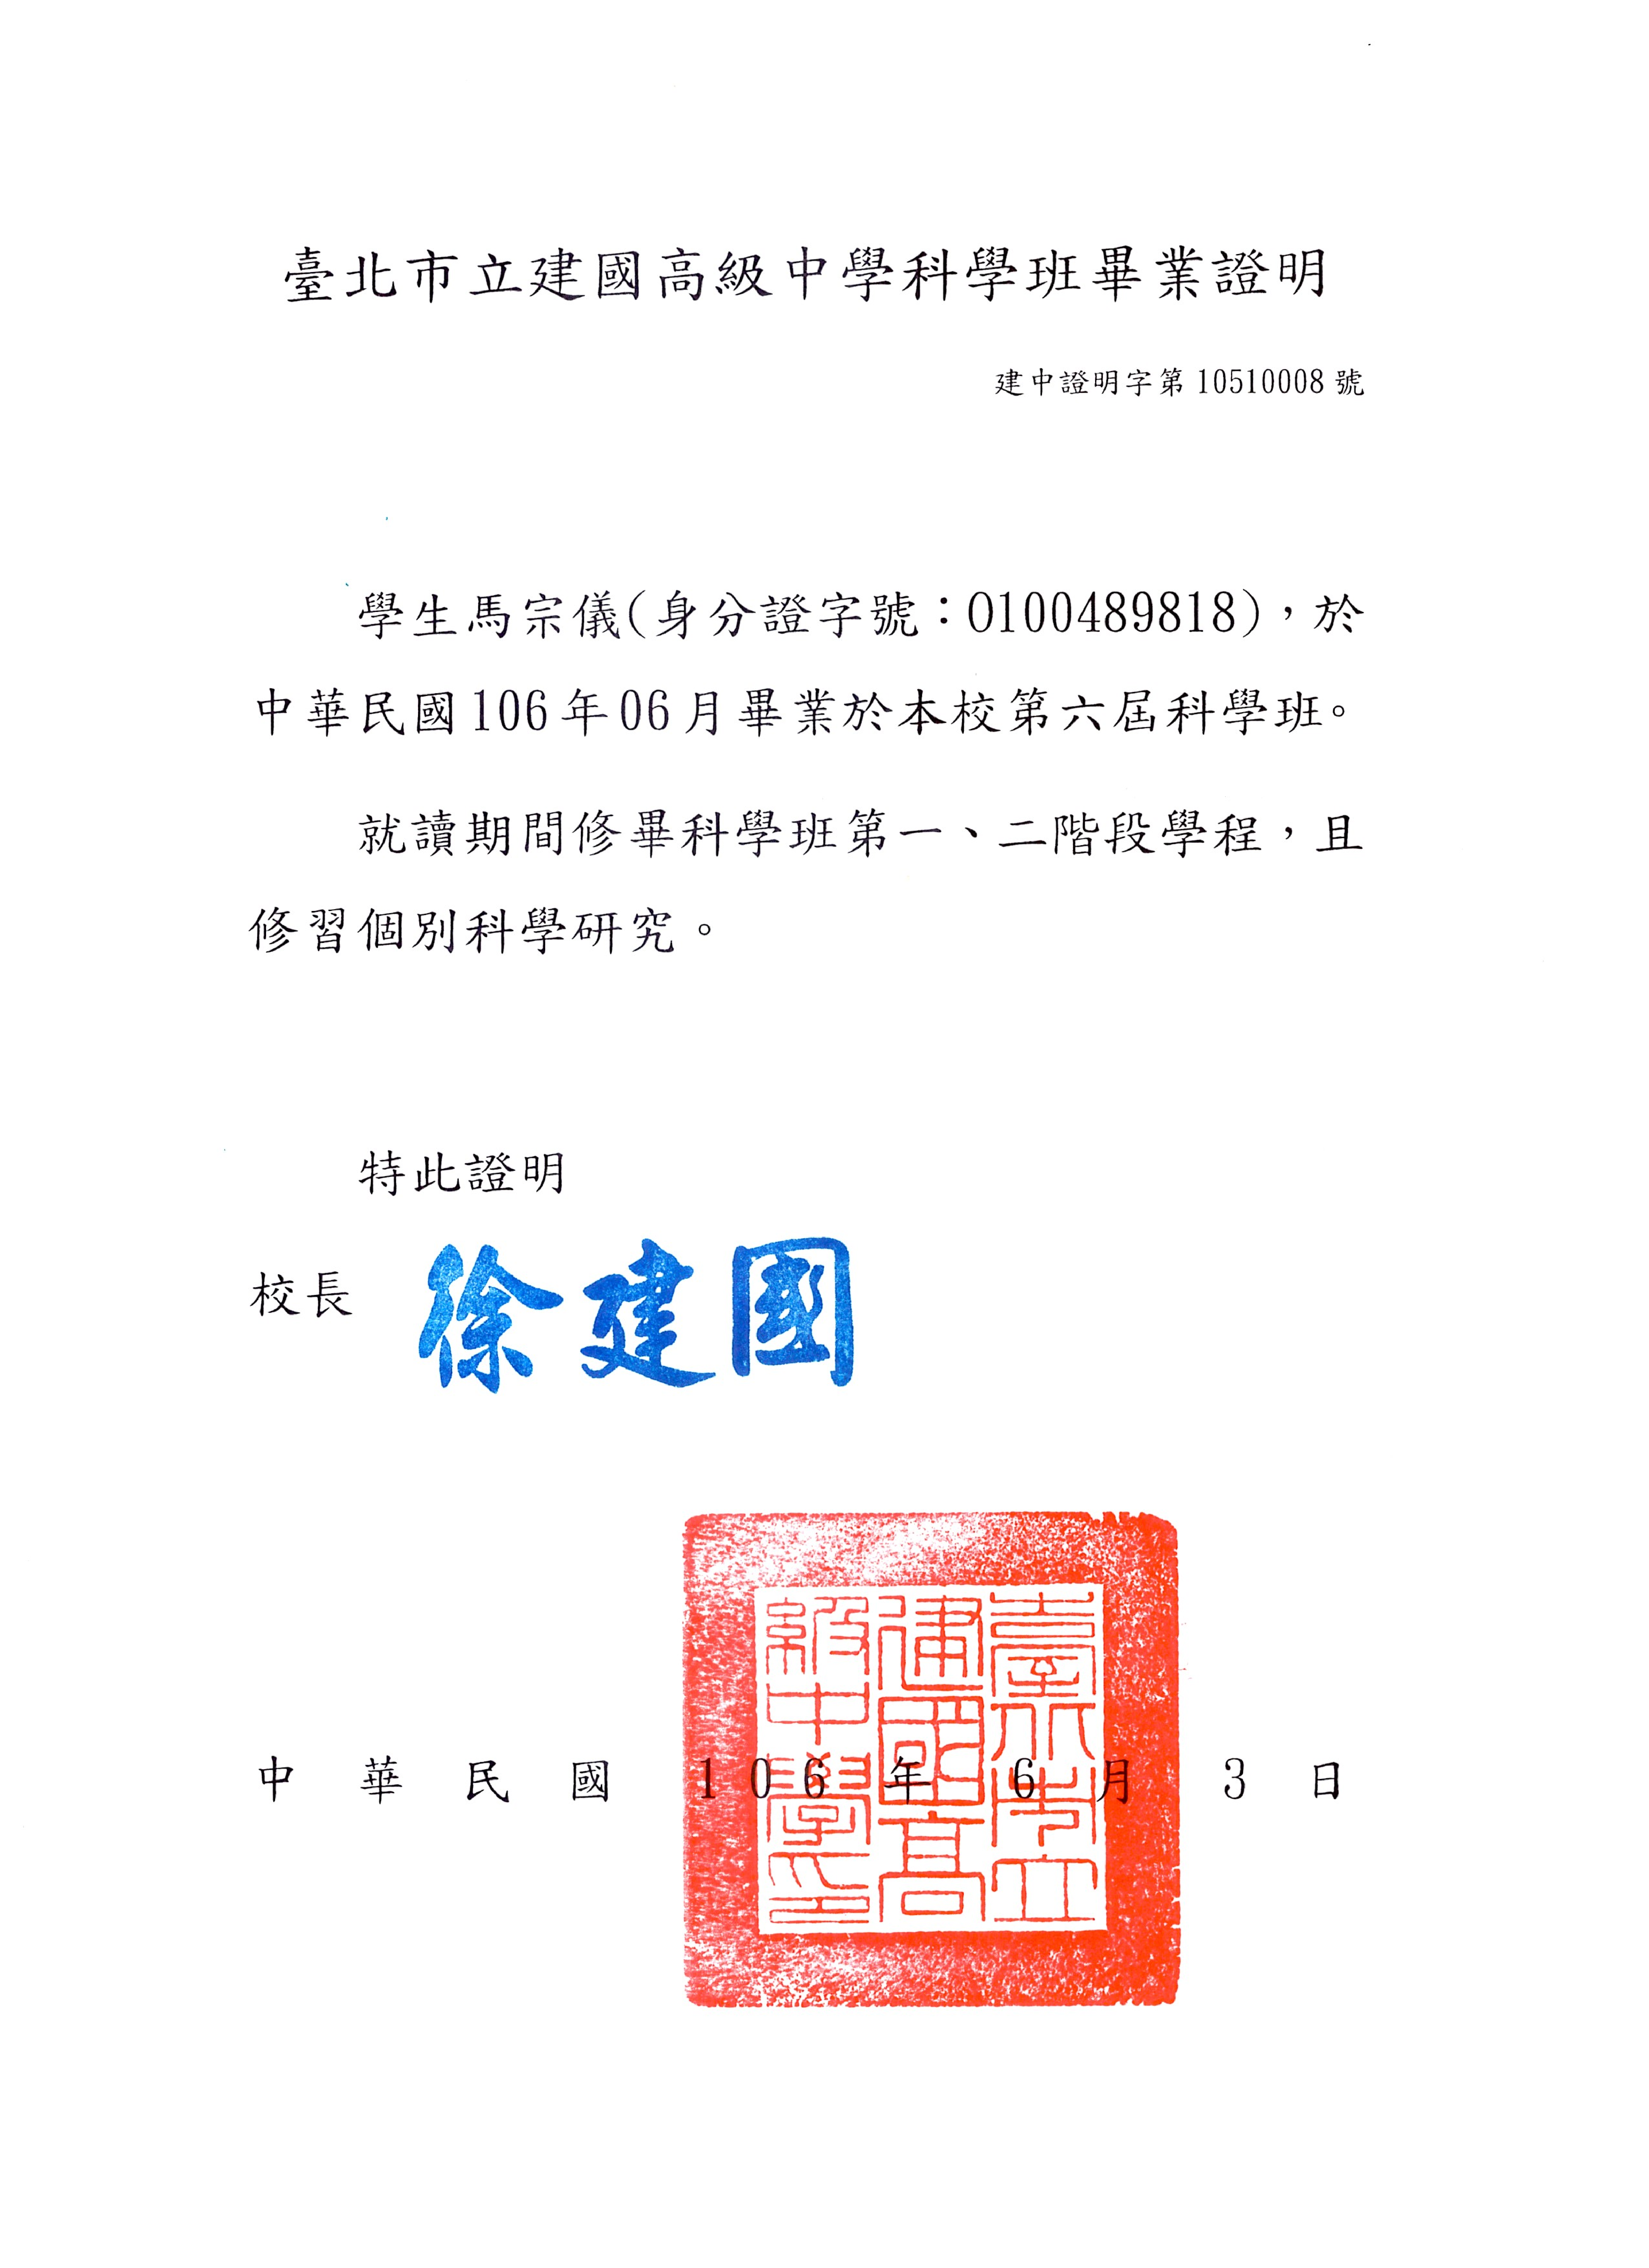
\includegraphics[page=1,width=0.32\textwidth,angle=90]{pdf_data/class_of_science.pdf}}
        \end{tabular}
    \end{center}
\end{document}